\normaltrue \difficilefalse \tdifficilefalse
\correctionfalse

%\UPSTIidClasse{11} % 11 sup, 12 spé
%\newcommand{\UPSTIidClasse}{12}
% ATS 2019
\exer{Suspension pneumatique de véhicule de transport routier$\star$ \label{A3:05:89}}
\setcounter{question}{0}
\marginnote{\xpComp{SYS}{01}}%\UPSTIcompetence[2]{A3-05}

\index{Compétence A3-05}
\index{Compétence SYS-01}
\index{Bouée}
\index{Caractériser un constituant de la chaîne de puissance}
\index{Distributeur}
\index{Vérin}
\ifcorrection
\else
\marginnote{\textbf{Pas de corrigé pour cet exercice.}}
\fi



\ifprof
\else
L’énergie produite à partir de la houle est appelée houlomotrice (ou énergie des vagues). Cette énergie est le plus souvent
transformée en énergie électrique.

\begin{marginfigure}
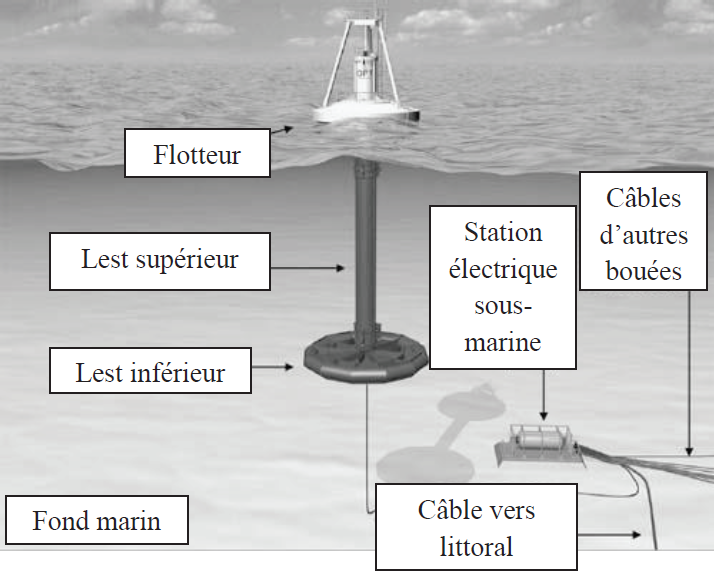
\includegraphics[width=\linewidth]{89_fig_01}
%\textit{}
\end{marginfigure}

Le système de conversion d'énergie est schématisé sur la figue suivante.

Le vérin hydraulique est entraîné par le mouvement relatif de translation entre le flotteur et le lest.
La translation du piston par rapport au cylindre du vérin est donc également paramétrée par le
déplacement $z(t)$ par rapport à la position d’équilibre. La section utile du piston est notée $S_p$. Les
pressions dans les chambres supérieure et inférieure du vérin sont notées respectivement $P_1$ et $P_2$.

Un réservoir accumulateur haute pression (a) et un réservoir accumulateur basse pression (b)
permettent de maintenir les pressions $P_a$ (pression d'admission du moteur hydraulique) et $P_b$
(pression de refoulement du moteur hydraulique) quasi-constantes en régime établi.

Un ensemble de clapets anti-retour permet de générer un débit volumique unidirectionnel $Q_m(t)$
vers le moteur hydraulique, quel que soit le sens de déplacement du piston. Les pertes induites par
ce circuit redresseur seront négligées. On pourra alors considérer en régime établi, et en première
approximation, les relations suivantes entre les pressions dans les réservoirs et dans les chambres du
vérin : $P_a = \text{max} \left(P_1,P_2\right)$ et $P_b = \text{min} \left(P_1,P_2\right)$.

\fi


\question{Compléter les zones en pointillés du schéma hydraulique en dessinant
les clapets anti-retour conformément à la description précédente.}
\ifprof
\begin{corrige}
\begin{center}
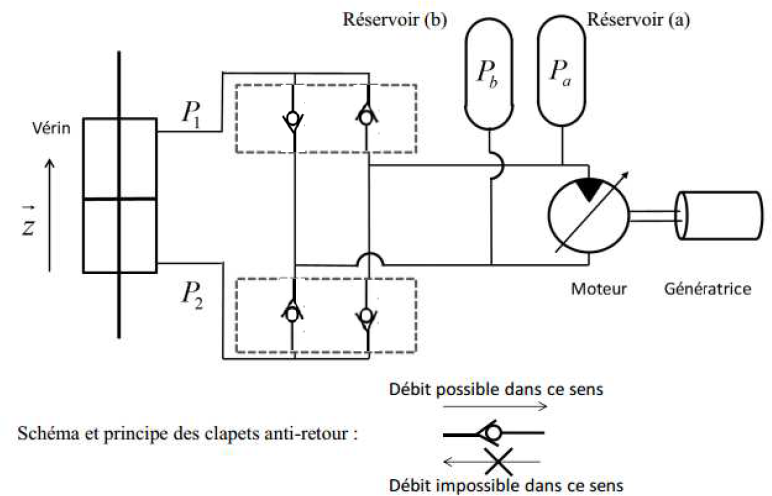
\includegraphics[width=.5\linewidth]{89_cor_01}
%\textit{}
\end{center}
\end{corrige}
\else

\begin{marginfigure}
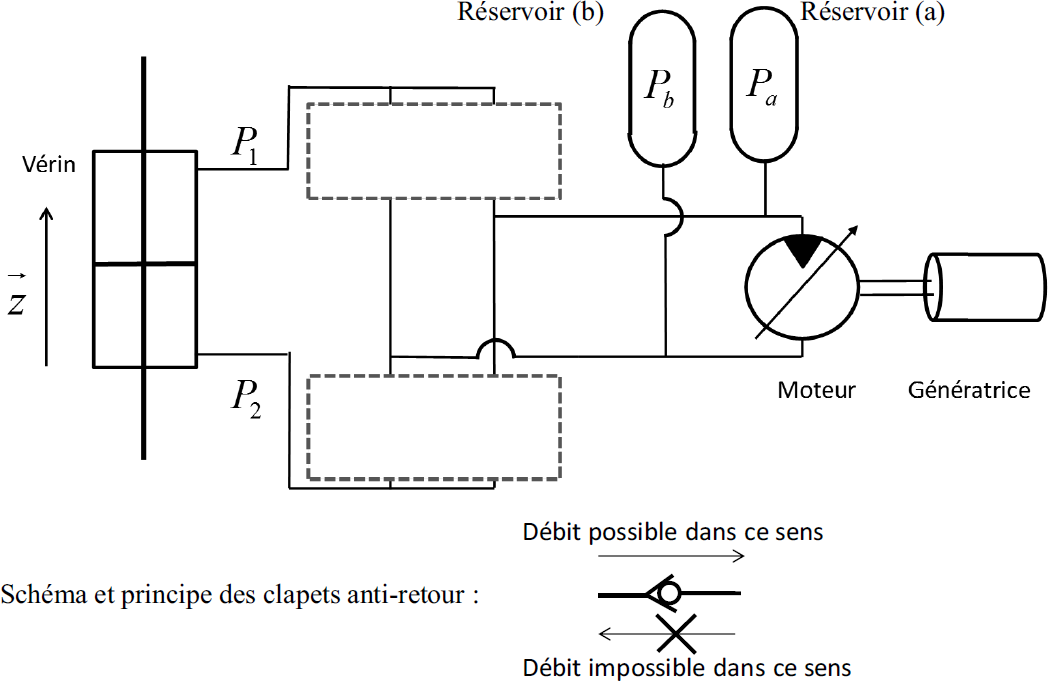
\includegraphics[width=\linewidth]{89_fig_02}
%\textit{}
\end{marginfigure}
\fi

\ifprof
\else
\begin{flushright}
\footnotesize{Corrigé  voir \ref{A3:05:89}.}
\end{flushright}%
\fi